\documentclass[article,A4,12pt]{llncs}
\usepackage[T1]{fontenc}
\usepackage{amsmath}
\usepackage{amssymb}
\usepackage{amsfonts}
\usepackage{mathrsfs, bm}

\usepackage{graphicx}
\usepackage{tabularx}
\usepackage{subfig}
\usepackage{epsf,times}
\usepackage{color}
\usepackage{wrapfig}
\usepackage{cases}
\usepackage{multicol}

\usepackage[T1]{fontenc}
%\newcommand{\tmname}[1]{\textsc{#1}}
%\newcommand{\tmop}[1]{\ensuremath{\operatorname{#1}}}
%\newcommand{\tmsamp}[1]{\textsf{#1}}
%\newcommand{\tmtextsc}[1]{{\scshape{#1}}}
%\newcommand{\tmtextsl}[1]{{\slshape{#1}}}
%\newcommand{\tmtexttt}[1]{{\ttfamily{#1}}}

\leftmargin=0.0cm
\oddsidemargin=0.5cm
\evensidemargin=0.5cm
\topmargin=0cm
\textwidth=16.0cm
%\textheight=21.5cm
\textheight=20.0cm
\pagestyle{plain}
\setlength{\columnsep}{20pt}

\def\m{\mathbf{m}}
\def\H{\mathbf{H}}
\def\E{\mathbf{E}}
\newcommand{\vepsi}{{\varepsilon}}
\def\hnorm#1#2{\vert\,#1\,\vert_{#2}}
\newcommand{\R}{{\mathbb R}}
\newcommand{\Sph}{{\mathbb S}}
\def\x{\mathbf{x}}
\def\hvec{\overline{\mathbf{h}}}
\def\evec{\overline{\mathbf{e}}}

\newcommand{ \etal}{\mbox{\emph{et al. }}}

\newcommand\vect[1]{\mbf{#1}}
\newcommand{\mbf}[1]{\mbox{\boldmath$#1$}} 
\newcommand{\RC}[1]{#1 $\times$ #1 $\times$ #1}
\def\um{$\mu$m}
\def\C{$^{\circ}\mathrm{C}$}

\newcommand{\Rmnum}[1]{\expandafter\@slowromancap\romannumeral #1@}

% DEFINITION OF CUSTOM FONT SIZE
\newcommand{\customfontA}{\fontsize{50}{55}\selectfont}
\newcommand{\customfontB}{\fontsize{14.4}{20}\selectfont}
\newcommand{\customfontC}{\fontsize{30}{35}\selectfont}

\DeclareMathAlphabet{\mathpzc}{OT1}{pzc}{m}{it}

\def\clovek#1{\noindent\bgroup\vbox{\noindent#1}\egroup\vskip1em}

% TO INPUT BACKGROUND IMAGE
\usepackage{eso-pic}
\newcommand\BackgroundPic{
\put(0,0){
\parbox[b][\paperheight]{\paperwidth}{
\vfill
\centering
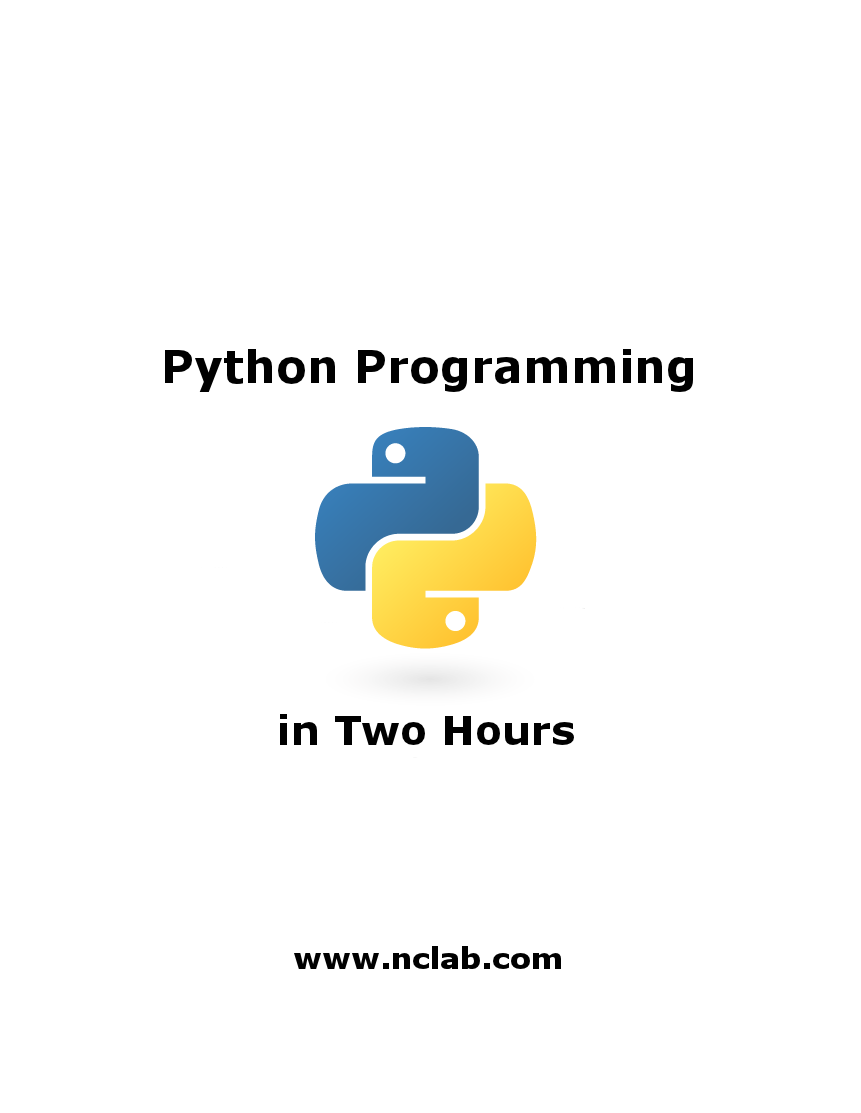
\includegraphics[width=\paperwidth,height=\paperheight]{img/python-frontpage.png}
%\includegraphics[width=\paperwidth,height=\paperheight]{img/background.jpg}
\vfill
}}}

\begin{document}

% INPUTTING BACKGROUND IMAGE
\AddToShipoutPicture{\BackgroundPic}
\vbox{}
\pagestyle{empty}
\newpage
\textwidth=15.5cm
\ClearShipoutPicture
\newpage

%%%%%%%%%%%%%%%%%%%%%%%%%%%%%%%%%%%%%%%%%%%%%%%%%%%%%%%%%%%%%%%%%%%%%%%%%

\section*{}
\small
\subsection*{About NCLab}
Networked Computing Laboratory (NCLab) is a popular Internet-based framework for 
programming, mathematics, computer modeling, 
and scientific computing. It serves students, instructors, researchers, and the general 
public. NCLab can be used free of charge for personal non-commercial purposes such as 
private hobby or self-education, as well as for individual non-funded academic research.
All other use is subject to {\bf purchasing a license} for a symbolic fee. The fees are as low as 
\$1 per user per month for educational use, and they are used to support the development 
and operational expenses. NCLab is a product of FEMhub Inc. The name "NCLab" is 
registered with the U.S. Patent and Trademark Office (USPTO) under Trademark No. 85420518.

\subsection*{Terms of Use and Pricing}
More details on purchasing a license and using NCLab are provided in the online documents 
{\bf Pricing} and {\bf Terms of Use} that are accessible from NCLab's home page 
{\tt http://nclab.com}.

\subsection*{Contact Information}
General inquiries: {\tt info@femhub.com}\\
Sales: {\tt sales@femhub.com}\\
NCLab support: {\tt support@nclab.com}\\
Agros \& Hermes support: {\tt support@femhub.com}\\
Web page: {\tt http://femhub.com}\\
{Physical address}\\
FEMhub Inc.\\
5490 Twin Creeks Dr.\\
Reno, NV 89523

\subsection*{About This Publication}
This publication can be copied and distributed without any restrictions
as long as reference to NCLab and FEMhub Inc. is preserved.

\subsection*{Acknowledgement}
This publication was created with the help of many freely 
available web resources related to Python, in
particular www.python.org.

\normalsize

\newpage
%{\ }
\setcounter{tocdepth}{2}
\tableofcontents
%\pagestyle{plain}

\newpage

\pagestyle{plain}
\setcounter{page}{1}

%%%%%%%%%%%%%%%%%%%%%%%%%%%%%%%%%%%%%%%%%%%%%%%%%%%%%%%%%%%%%%%%%%%%%%%%%

\section{Introduction}

Python is a modern, powerful programming language that is also very intuitive and 
easy to learn. It has efficient high-level 
data structures and a simple but effective approach to object-oriented programming. 
Python's elegant syntax and dynamic typing, together with its interpreted nature, 
make it an ideal language for beginners. 
In this short course you will 
learn the most important aspects of the language and be able to 
write a wide range of programs by yourself. Depending on your objectives, this course 
might be all you will ever need. We hope that you will like Python and want
to learn more -- and there is much more to learn out there. References to materials
covering more advanced topics and object-oriented programming are given in Section \ref{sec:adv}.

In order to make the most of this tutorial, create an account in NCLab and log in. More instructions 
on how to do this are given at the beginning of the introductory 
tutorial "Meet Your New Graphing Calculator" that is available in 
PDF from NCLab's home page {\tt http://nclab. com}.
After login, you will see a desktop with several icons on it,
as shown in Fig. \ref{fig:desktop}. 


\begin{figure}[!ht]
\begin{center}
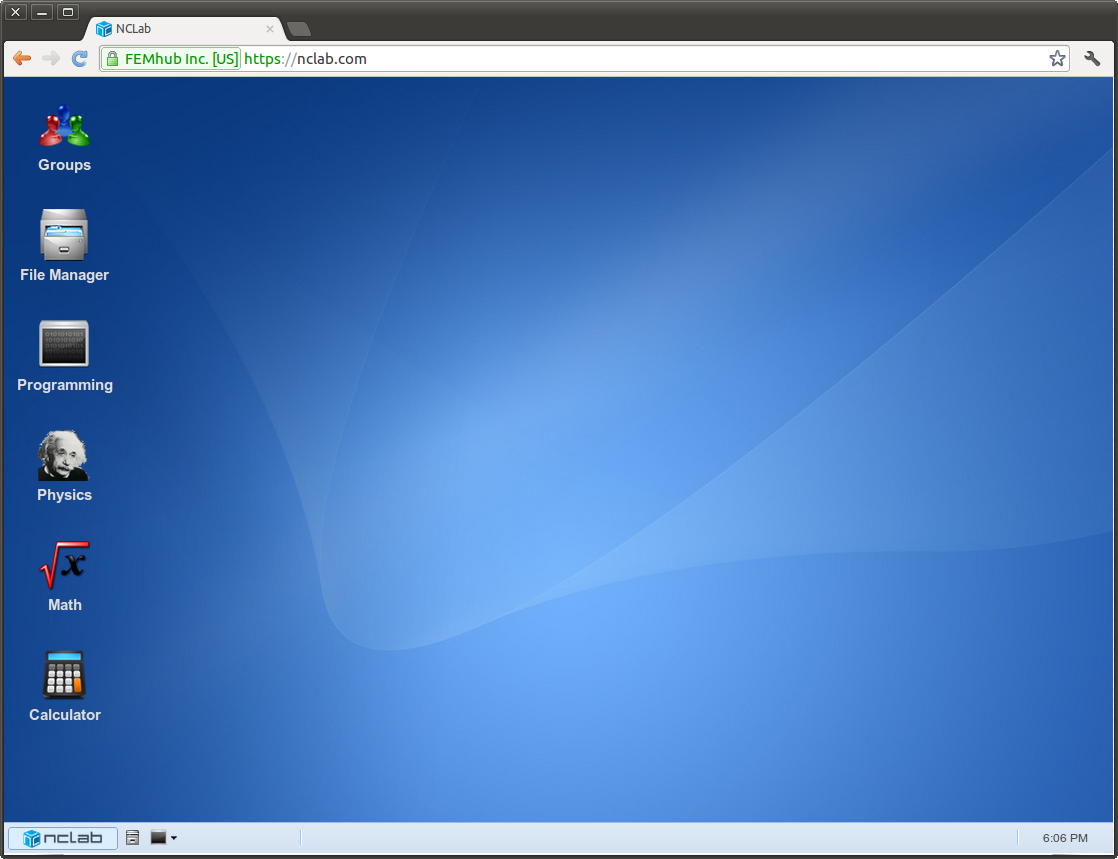
\includegraphics[width=0.8\textwidth]{img/desktop.png}
\end{center}
\vspace{-2mm}
\caption{NCLab desktop after login.}
\label{fig:desktop}
\end{figure}
\newpage

\subsection*{Cloning Displayed Projects vs. Typing the Code by Yourself}

All examples that we are going to work with in the following are also available 
as Displayed Projects. This means that you can clone them by launching the File
Manager, going to the {\em Project} menu, and clicking on {\em Clone}. This will launch 
a window with many displayed projects from various areas of programming,
math and computing. Look for projects whose names start with "Tutorial - Python".
After you locate a project that you would like to clone, click on it,
and then click on the button {\em Clone} at the bottom of the window. This will
create exact copy of that project in your account, and you can open it 
by clicking on it in the File Manager. You can change the project in any way 
you like, the changes will not affect the original Displayed Project. 

Alternatively, you can type the examples by yourself, which is the 
recommended way. What you do with your own hands will come back much easier 
when you do it again. And moreover, the introductory examples have no more than 
a couple of lines anyway. So, in the File Manager's {\em Project} menu 
choose {\em New} $\rightarrow$ {\em Python}. This will launch an 
empty Python project, as shown in Fig. \ref{fig:python}.\\[-7mm]


\begin{figure}[!ht]
\begin{center}
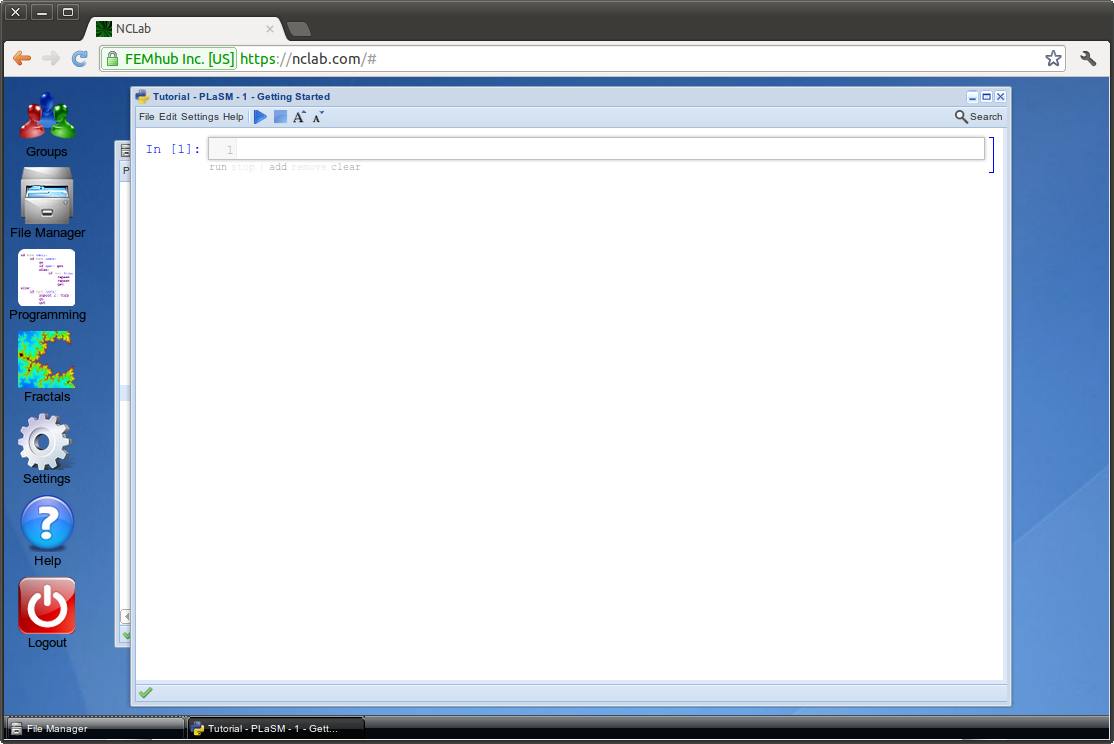
\includegraphics[width=0.8\textwidth]{img/python.png}
\end{center}
\vspace{-2mm}
\caption{Launching a new Python project.}
\label{fig:python}
\end{figure}
\vspace{-1cm}
\noindent
\newpage

\section{Hello, World!}

Click into the input cell and type {\tt print "Hello, World!"}.
Then click on the "run" link under the input cell and your program will be sent to the 
cloud. The response should come back instantly, and it should be displayed 
in a new yellow {\em output cell} as shown in Fig. \ref{fig:python-2}.\\[-7mm]

\begin{figure}[!ht]
\begin{center}
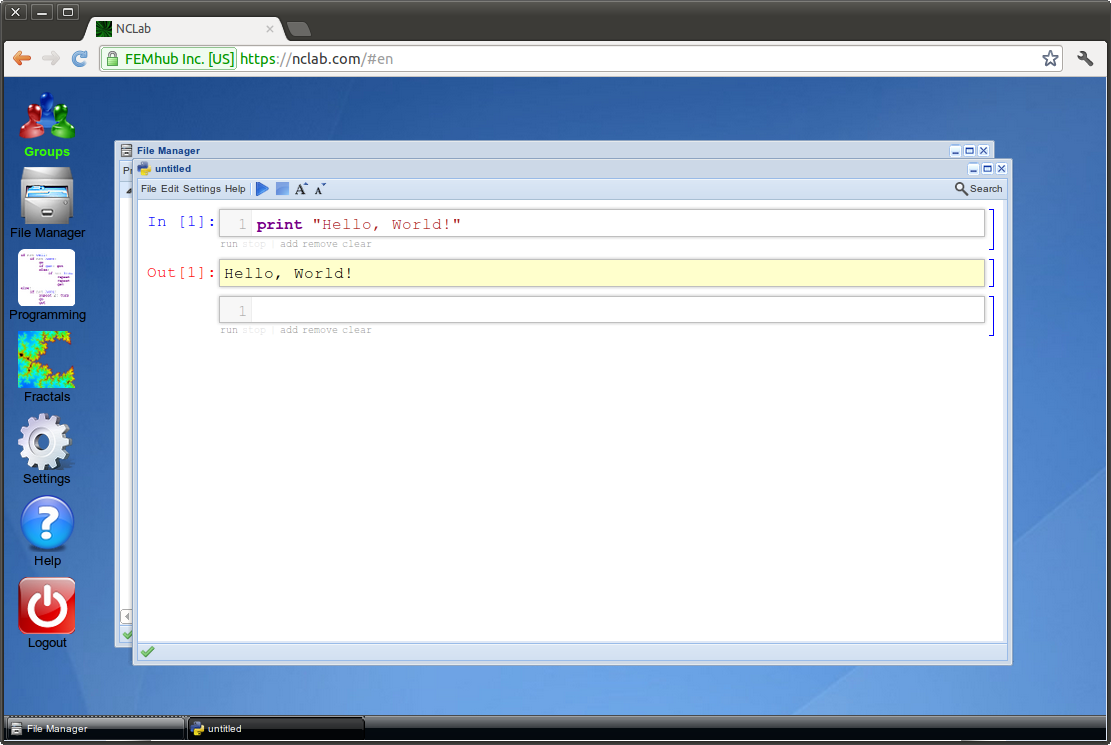
\includegraphics[width=0.8\textwidth]{img/python-2.png}
\end{center}
\vspace{-2mm}
\caption{Response received from the cloud is shown in a yellow output cell.}
\label{fig:python-2}
\end{figure}
%\vspace{-1cm}
\noindent
You just learned the first Python command. Wasn't that simple?

\section{Numbers}

The Python input cell can be used as a calculator. Try it and type 

\begin{verbatim}
3 + 6
\end{verbatim}
The click on the "run" link under the input cell. (We will not repeat the last sentence 
in the following, since this is the same whenever we want to send the contents of the input 
cell to the cloud.) The output is

\begin{verbatim}
9
\end{verbatim}
You can add real numbers too,
\begin{verbatim}
3.2 + 6.31
\end{verbatim}
Output:

\begin{verbatim}
9.51
\end{verbatim}
Two numbers can be subtracted as follows,

\begin{verbatim}
7.5 - 2.1
\end{verbatim}
Output:

\begin{verbatim}
5.4
\end{verbatim}
Multiplication is done using the '{\tt *}' symbol as in

\begin{verbatim}
3 * 12
\end{verbatim}
Output:

\begin{verbatim}
36
\end{verbatim}
Of course, real numbers can be multiplied as well:

\begin{verbatim}
3.7 * 12.17
\end{verbatim}
Output:

\begin{verbatim}
45.029
\end{verbatim}
With division, we need to be a bit careful. Look at this:

\begin{verbatim}
30 / 5
\end{verbatim}
Output:

\begin{verbatim}
6
\end{verbatim}
And then look at this:

\begin{verbatim}
33 / 5
\end{verbatim}
Output:

\begin{verbatim}
6
\end{verbatim}
In all major computer languages including C, C++, Fortran, Python and 
others, {\bf the result of division of two integers is an integer}. 
So, when dividing two integers, everything behind the decimal point is lost.
In fact this is true also for addition, subtraction and multiplication 
but there it cannot cause any harm. 

In order to stay on the safe side, 
before you perform division of two numbers, always convert at least one of them
to a real number. This is simple: While {\tt 5} is an integer, {\tt 5.}
and {\tt 5.0} are reals. It is also possible to 
say {\tt float(5)}. In fact this is the best way since it also works for 
variables. Such as, when we are dividing {\tt a / b}, to make sure that 
the result will be correct also for integers, we type {\tt float(a) / b}. 
When at least one number is a real, then the result of the division is a real.   
Variables will be discussed shortly.

Sometimes we need to use exponents, such as in $2^4$. Python has a double-star
symbol {\tt **} for this:

\begin{verbatim}
2**4
\end{verbatim}
Output:

\begin{verbatim}
16
\end{verbatim}
The last of the common arithmetic operations is {\em modulo}. Recall that this is the remainder 
after integer division. In Python modulo is done using the per cent symbol:

\begin{verbatim}
6 % 4
\end{verbatim}
Output:

\begin{verbatim}
2
\end{verbatim}
Of course, one can use brackets:

\begin{verbatim}
5 * (7 - 3)
\end{verbatim}
Output:

\begin{verbatim}
20
\end{verbatim}
Python respects the standard order of operations:

\begin{itemize} 
\item Brackets have the highest priority, 
\item then exponentiation, 
\item then multiplication and division (same priority),
\item the lowest priority have addition and subtraction.
\end{itemize}
To illustrate this, we can try the following:

\begin{verbatim}
3**4/27*5+3*5
\end{verbatim}
Output:

\begin{verbatim}
30
\end{verbatim}
Let us remark that your code will be much more readable when you use empty
characters on either side of arithmetic symbols. Hence instead of the 
previous compact expression you should write {\tt 3**4 / 27 * 5 + 3 * 5}.

Complex numbers are always represented as two floating point numbers, the 
real and imaginary part. Appending '{\tt j}' or  '{\tt J}' to a real number
makes it imaginary:

\begin{verbatim}
1j * 1J
\end{verbatim}
Output:

\begin{verbatim}
(-1+0j)
\end{verbatim}
This is one way to define complex numbers:
\begin{verbatim}
1 + 3j
\end{verbatim}
Output:

\begin{verbatim}
(1+3j)
\end{verbatim}
Another way is to use the command {\tt complex}:

\begin{verbatim}
complex(1, 3)
\end{verbatim}
Output:

\begin{verbatim}
(1+3j)
\end{verbatim}
All arithmetic operations that are used for real numbers can be 
used for complex numbers as well, for example:

\begin{verbatim}
(1 + 2j) / (1 + 1j)
\end{verbatim}
Output:

\begin{verbatim}
(1.5+0.5j)
\end{verbatim}
To extract the real and imaginary parts of a complex number {\tt z}, use {\tt z.real}
and {\tt z.imag}. Use {\tt abs()} to get the absolute value:

\begin{verbatim}
a = 3 + 4j
a.real
a.imag
abs(a)
\end{verbatim}
Output:

\begin{verbatim}
3
4
5
\end{verbatim}
Good job, now you know your numbers!

\section{Variables}

In Python (and other languages as well) the symbol '{\tt =}' is used to assign 
a value to a variable. This operation does not produce any output. For
example:

\begin{verbatim}
width = 20
height = 5*5
\end{verbatim}
Output:

\begin{verbatim}

\end{verbatim}
(Yes, there is none!) If we want to see the values, we need to print the 
variables. To do this, it suffices to type the variable's name:

\begin{verbatim}
width
height
\end{verbatim}
Output:

\begin{verbatim}
20
25
\end{verbatim}
Or, we can use the print command:

\begin{verbatim}
print width
print height
\end{verbatim}
Output:

\begin{verbatim}
20
25
\end{verbatim}
The output can be made more informative (strongly encouraged!):

\begin{verbatim}
print "The width of the object is", width
print "And its height is", height
\end{verbatim}
Output:

\begin{verbatim}
The width of the object is 20
And its height is 25
\end{verbatim}
A value can be assigned to several variables at the same time:

\begin{verbatim}
x = y = z = 0.0
x
y
z
\end{verbatim}
Output:

\begin{verbatim}
0.0
0.0
0.0
\end{verbatim}
Variables must be defined (have a value assigned) before they can be 
used. For example, when trying to print a variable {\tt value} that 
was never used before, we get an error:

\begin{verbatim}
Traceback (most recent call last):
  File "<nclab>", line 1, in <module>
NameError: name 'value' is not defined
\end{verbatim}
The simplest way to increase the value of a variable by a given number is to use the '{\tt +=}' 
command:

\begin{verbatim}
v = 1
v += 3
print v
\end{verbatim}
Output:

\begin{verbatim}
4
\end{verbatim}
We can also subtract a number from a variable:

\begin{verbatim}
print v -= 1
\end{verbatim}
Output:

\begin{verbatim}
3
\end{verbatim}
We can multiply a variable with a number:

\begin{verbatim}
print v *= 4
\end{verbatim}
Output:

\begin{verbatim}
12
\end{verbatim}
And finally, we can divide a variable with a number:

\begin{verbatim}
print v /= 6
\end{verbatim}
Output:

\begin{verbatim}
2
\end{verbatim}
It is possible to use existing variables to assign a value to a new variable:

\begin{verbatim}
a = 1
b = 2.5
c = 0.5
d = (a + b) / c
d
\end{verbatim}
Output:

\begin{verbatim}
7.0
\end{verbatim}
And this lucky number means the end of this section!

\section{Strings}

By a {\em string} we mean a text surrounded by double or single quotes, such as 
{\tt "this is a string"} or {\tt 'and this is a string as well'}.
Strings are useful to make outputs more informative, but 
they have many other uses as well. For example, they can represent data 
in databases such as in a phone book. So we need to understand them well,
as well as various operations that we can do with them.

Let us first understand how to use quotes in strings. The safest way is to use 
them with a backslash:

\begin{verbatim}
"I said \"yes\"."
\end{verbatim}
Output:

\begin{verbatim}
'I said "yes".'
\end{verbatim}
Another example:

\begin{verbatim}
"It doesn\'t matter."
\end{verbatim}
Output:

\begin{verbatim}
"It doesn't matter."
\end{verbatim}
When we want to use multi-line strings, the best way is to enclose them 
in triple quotes:

\begin{verbatim}
edgar = """
Once upon a midnight dreary, while I pondered weak and weary,
Over many a quaint and curious volume of forgotten lore,
While I nodded, nearly napping, suddenly there came a tapping,
As of some one gently rapping, rapping at my chamber door.
`'Tis some visitor,' I muttered, `tapping at my chamber door -
Only this, and nothing more.'
"""
print edgar
\end{verbatim}
Output:

\begin{verbatim}
Once upon a midnight dreary, while I pondered weak and weary,
Over many a quaint and curious volume of forgotten lore,
While I nodded, nearly napping, suddenly there came a tapping,
As of some one gently rapping, rapping at my chamber door.
`'Tis some visitor,' I muttered, `tapping at my chamber door -
Only this, and nothing more.'
\end{verbatim}
Strings can be concatenated (glued together) with the '{\tt +}' operator, and repeated with '{\tt *}':

\begin{verbatim}
word = 'Help' + 'me!'
print "I yelled" + 3 * word
\end{verbatim}
Output:

\begin{verbatim}
I yelledHelpme!Helpme!Helpme!
\end{verbatim}
You can see that empty spaces matter. Let's try again:

\begin{verbatim}
word = '\"Help' + ' me!\" '
print "I yelled " + 3 * word
\end{verbatim}
Output:

\begin{verbatim}
I yelled "Help me!" "Help me!" "Help me!"
\end{verbatim}
Individual letters forming a string can be accessed via indices. The indices 
start from zero, as in C and C++. It is also handy to use the index {\tt -1} 
for the last index, {\tt -2} for the one-before-last etc.


\begin{verbatim}
word = "breakfast"
print "First character:", word[0]
print "Second character:", word[1]
print "Last character:", word[-1]
print "One-before-last character:", word[-2]
\end{verbatim}
Output:

\begin{verbatim}
First character: b
Second character: r
Last character: t
One-before-last character: s
\end{verbatim}
We can also access substrings, this is called {\em slicing}:

\begin{verbatim}
w1 = "bicycle"
w2 = w1[0:3]
print w2
\end{verbatim}
Output:

\begin{verbatim}
bic
\end{verbatim}
An omitted first index in a slice defaults to zero:

\begin{verbatim}
w3 = w1[0:2]
print w3
\end{verbatim}
Output:

\begin{verbatim}
bi
\end{verbatim}
An omitted second index defaults to the length of the string:

\begin{verbatim}
w4 = w1[2:]
print w4
\end{verbatim}
Output:

\begin{verbatim}
cycle
\end{verbatim}
And by the way, the length of a string can be obtained via the {\tt len()} function:

\begin{verbatim}
print len(w1)
\end{verbatim}
Output:

\begin{verbatim}
7
\end{verbatim}
Perhaps this lesson could be longer but it isn't!

\section{Boolean expressions}

Boolean expressions are the foundation of every procedural programming 
language including Python. Remember how the value of a variable 
is assigned and printed? 

\begin{verbatim}
a = 1
a
\end{verbatim}
Output:

\begin{verbatim}
1
\end{verbatim}
Now type

\begin{verbatim}
a > 0
\end{verbatim}
Output:

\begin{verbatim}
True
\end{verbatim}
And,

\begin{verbatim}
a < 0
\end{verbatim}
Output:

\begin{verbatim}
False
\end{verbatim}
Conditions {\tt a > 0} and {\tt a < 0} are {\em Boolean expressions} whose value is either 
{\tt True} or {\tt False}. Conditions related to numbers often contain the following operators:

\begin{itemize}
\item[(1)] {\tt >} {$\ldots$} greater than, 
\item[(2)] {\tt >=} {$\ldots$} greater than or equal to, 
\item[(3)] {\tt <=} {$\ldots$} less than or equal to, 
\item[(4)] {\tt <} {$\ldots$} less than, 
\item[(5)] {\tt ==} {$\ldots$} equal to, 
\item[(6)] {\tt !=} {$\ldots$} not equal to, 
\item[(7)] {\tt <>} {$\ldots$} not equal to (same as {\tt !=}).
\end{itemize}
We can store the value of a Boolean expression in a variable:

\begin{verbatim}
v1 = (a > 0)
v1
\end{verbatim}
Output:

\begin{verbatim}
True
\end{verbatim}
Such variable {\tt v1} is called {\em Boolean variable}. With Boolean variables we can do all standard 
logical operations such as {\tt and}:

\begin{verbatim}
v2 = (a < 5)
v1 and v2
\end{verbatim}
Output:

\begin{verbatim}
True
\end{verbatim}
Logical {\tt or}:

\begin{verbatim}
v3 = (a > 10)
v1 or v3
\end{verbatim}
Output:

\begin{verbatim}
True
\end{verbatim}
Negation:

\begin{verbatim}
v4 = not v1
v4
\end{verbatim}
Output:

\begin{verbatim}
False
\end{verbatim}
Sometimes logical expressions can be more complicated, but this is no problem:

\begin{verbatim}
v5 = not ((v1 and v2) or (v3 and not v4))
v5
\end{verbatim}
Output:

\begin{verbatim}
False
\end{verbatim}
Last let us type

\begin{verbatim}
v6 = not v5
\end{verbatim}
to end this section in a positive way!

\section{Conditions}

Each procedural programming language including Python enables conditional 
execution of code. What does this mean? Imagine that you have to write
a program to calculate
$$
\frac{1}{9 - x^2}
$$
for any value of $x$. Of course, this is simple:

\begin{verbatim}
result = 1. / (9 - x**2)
print "Result is", result
\end{verbatim}
However, when a user calls your program with $x = 3$ or $x = -3$, then
it crashes!

\begin{verbatim}
Traceback (most recent call last):
  File "<nclab>", line 1, in <module>
ZeroDivisionError: float division by zero
\end{verbatim}
This is not a good thing to happen, and thus we need to be more careful.
Here is an alternative version of the program that will not crash:

\begin{verbatim}
if (x == 3) or (x == -3):
    print "Result is undefined, division by zero!"
    result_defined = False
else:
    result = 1. / (9 - x**2)
    print "Result is", result
    result_defined = True
\end{verbatim}
Notice that the lines in the {\tt if} and {\tt else} branches are indented,
The indent means that a command is still inside the {\tt if} or {\tt else}
branch.

Failure to use indents properly will result into an incorrect program. For 
example, if we forgot to indent the last line in the above program,

\begin{verbatim}
if (x == 3) or (x == -3):
    print "Result is undefined, division by zero!"
    result_defined = False
else:
    result = 1. / (9 - x**2)
    print "1 / (9 - x**2) =", result
result_defined = True
\end{verbatim}
then the last line would be outside of the {\tt if - else} statement, and
thus the variable {\tt result\_ defined} would be always {\tt True}!\\

\noindent
Sometimes the {\tt else} branch is not needed, and in that case it can be omitted:

\begin{verbatim}
if (x != 3) and (x != -3):
    result = 1. / (9 - x**2)
    print "Result is", result
    result_defined = True
\end{verbatim}
Sometimes we need to consider more cases. For this, we can use {\tt elif}
(abbreviation for "else if"):

\begin{verbatim}
if (x == 3) or (x == -3):
    print "Result is undefined, division by zero!"
elif abs(x) < 3:
    print "Result is positive."
else:
    print "Result is negative."
\end{verbatim}
There can be more {\tt elif} statements if needed. \\

\noindent
In more complicated cases, conditions can be embedded in other conditions:

\begin{verbatim}
if (x == 3) or (x == -3):
    print "Result is undefined, division by zero!"
elif abs(x) < 3:
    if x < 0:
        print "x is negative and result is positive."
    else: 
        print "x is positive and result is positive."
else:
    if x < 0:
        print "x is negative and result is negative."
    else: 
        print "x is positive and result is negative."
\end{verbatim}
If your head hurts, do not worry. This section is over 
and the next one is going to be simpler!

\section{The {\tt while} loop}\label{sec:while}

Loops are a powerful tool as they allow us to use the computer to solve
tasks that would take many hours, months, or even years to a human person. 
Let's do something really simple. We know that the sine and cosine functions 
intersect somewhere between $x = 0$ and $x = \pi/2$. Let's make this more accurate!

\begin{verbatim}
from numpy import sin, cos
x = 0
dx = 1e-6
while cos(x) - sin(x) > 0:
    x += dx    
print "Result is approximately", x
\end{verbatim}
Output:

\begin{verbatim}
Result is approximately 0.785399000002
\end{verbatim}
In other words, the {\tt while} loop run 785399 times before 
the function $\cos(x) - \sin(x)$ flipped the sign! Can you 
imagine doing this on your pocket calculator?

The above program deserves some more comments: First, the sine and cosine 
functions are imported from the Numpy library. Using libraries 
is a standard part of Python programming. In particular, Numpy 
is a large collection of numerical algorithms and functions, and 
more about it will be said in Section \ref{subsec:importinglib},
Second, there are much more sophisticated algorithms for solving 
the equation $\cos(x) - \sin(x) = 0$ numerically, such as the Newton's 
method. These are also available in Numpy.

The body of the {\tt while} loop needs to be indented, similarly as
the bodies of the {\tt if} and {\tt else} statements. The body of
the {\tt while} loop
is repeated as long as the condition behind the keyword {\tt while}
is satisfied. If it is not satisfied the first time, the entire 
loop is skipped. 

It is typical for {\tt while} loops that the condition contains 
an expression that depends on a variable that is changed inside the 
loop. This was the case in the above program as well. In other 
words, we use the {\tt while} loop {\bf if we do not know the number of 
repetitions in advance.} If we know that something needs to be done
a known number of times (such as 1000 times), we use the {\tt for} loop.
The {\tt for} loop will be discussed in Section \ref{sec:forloop}.\\

\noindent
This section is finished, good job!

\section{Defining new functions}

Functions are little self-contained programs that perform a specific task, 
which you can incorporate into your own, larger programs. After you have 
created a function, you can use it at any time, in any place. This saves you 
the time and effort of having to retell the computer what to do every time 
it does a common task. 

For example, let's write a function that will look for a character {\tt c} 
in a string {\tt s}. If the character is found, it will return its index. 
If not, it will return -1. The definition of a new function 
is done via the reserved word {\tt def}:

\begin{verbatim}
# Finds the first occurence of a given character in a given 
# string, and returns its position. If not found, returns -1. 
def find_char(c, s):
    if len(c) != 1: 
        print "c must be a single character!"
        return -2
    n = 0
    while s[n] != c:
        n += 1
        if n == len(s):
            return -1
    return n
\end{verbatim}
Again, some remarks are in order. First of all notice the comment after the 
symbol '{\tt \#}'. Any text behind this symbol till the end of line is ignored 
by the interpreter, and thus one can use it for descriptions. {\bf Writing 
comments is strongly encouraged}. They make your program more readable for others
{\em and also for you}. Keep in mind that everything is perfectly clear to you 
at the time you are writing the program. But when you return to it in 6 months, 
without good comments you will have a hard time to remember why you wrote that 
function, and what exactly it was supposed to do. 

Second -- humans make mistakes. Whenever a function is to be used by a human
and it assumes something (such as that {\tt c} is a single character), {\bf check
it}. This means to write some extra code, but this extra effort pays off big time.
The user may not be a bad person who intentionally wants to crash your 
code (although there are such people!), but people do not read instructions, 
forget them, and can make a variety 
of mistakes. Sometimes these tests are called {\em sanity checks} -- basically
making sure that the function received correct data.

Third -- whenever there is 
a situation where your code can crash, check the input. If something is wrong,
do not let the program crash and rather {\bf take care of the problem youself}. 
Give the user (or yourself) a message that something happened in the program that 
was not supposed 
to happen. It saves you many a headache and lots of time wasted by going through 
your code and trying to find out why it does not work as expected. This is called 
{\em debugging} and for beginners it typically takes more time than writing the 
code itself. An example, bad code first:

\begin{verbatim}
from numpy import sqrt
...
a = sqrt(x)
\end{verbatim}
(here {\tt sqrt()} is the square root function and we import it from Numpy). If
for any reason {\tt x} is negative at the moment the square root is calculated,
the program crashes. So a better code is:

\begin{verbatim}
from numpy import sqrt
....
if x > 0:
    a = sqrt(x)
else:
    print "Sqrt(x) attempted with x =", x
    ...
\end{verbatim}
The second triple dots stand for an action that you take when incorrect 
input for the {\tt sqrt()} function is detected. What you do depends on 
your code -- for example you can skip this value of {\tt x} and calculate 
with the next one. 

\section{Tuples}

Sometimes we need to store data that does not change in time - such as 
the names of weekdays, or names of months. For this we use {\em tuples}.
To define a tuple, enclose comma-separated items in round brackets: 

\begin{verbatim}
months = ('January', 'February', 'March', 'April', 'May', 'June',\
'July', 'August', 'September', 'October', 'November', 'December')
\end{verbatim}
The items in the tuple {\tt months} are all strings, but this does not 
have to be. A tuple can be very heterogeneous -- it can contain strings,
numbers, other tuples, etc. Although -- in simplicity is beauty, we
do not have to always take advantage of the extreme possibilities.
It is important to remember that {\bf a tuple, once defined, cannot 
be changed} in the sense that no new items can be added and existing 
items cannot be deleted.

Items in a tuple are referenced by indices pretty much as characters 
are referenced in a string:

\begin{verbatim}
print "First month:", months[0]
print "Second month:", months[1]
print "Third month:", months[2]
print "Last month:", months[-1]
\end{verbatim}
Output:

\begin{verbatim}
First month: January
Second month: February
Third month: March
Last month: December
\end{verbatim}
We can also {\em slice} tuples similarly to how we sliced strings:

\begin{verbatim}
months[2:5]
\end{verbatim}
Output:

\begin{verbatim}
('March', 'April', 'May')
\end{verbatim}
The length of a tuple is obtained using the function {\tt len()}:

\begin{verbatim}
len(months)
\end{verbatim}
Output:

\begin{verbatim}
12
\end{verbatim}
Tuples become especially useful in combination with the {\tt for}
loop that will be discussed in Section \ref{sec:forloop}. 

\section{Lists}

\noindent
Lists are similar to tuples, and all indexing and slicing works in the same way. 
The biggest difference between a tuple 
and a list is that {\bf items in a list can be changed}. So, we use
lists for items that can change in time. Let's say that there are 
10 people in a school class {\tt cls}:

\begin{verbatim}
cls = ['John', 'Pam', 'Emily', 'Jessie', 'Brian', \
'Sam', 'Jim', 'Tom', 'Jerry', 'Alex']
\end{verbatim}
Then however, Emily moves to a different city:

\begin{verbatim}
del cls[2]
print cls
\end{verbatim}
Output

\begin{verbatim}
['John', 'Pam', 'Jessie', 'Brian', 'Sam', 'Jim', 
'Tom', 'Jerry', 'Alex']
\end{verbatim}
After some time, a new student Jack moves in:

\begin{verbatim}
cls.append('Jack')
print cls
\end{verbatim}
Output

\begin{verbatim}
['John', 'Pam', 'Jessie', 'Brian', 'Sam', 'Jim', 
'Tom', 'Jerry', 'Alex', 'Jack']
\end{verbatim}
Useful can be the function {\tt pop()} that deletes an item and returns it for further
use (as opposed to {\tt del} which just deletes the item):

\begin{verbatim}
name = cls.pop(2)
print name 
print cls
\end{verbatim}
Output

\begin{verbatim}
Jessie
['John', 'Pam', 'Brian', 'Sam', 'Jim', 
'Tom', 'Jerry', 'Alex', 'Jack']
\end{verbatim}
New item can be inserted at an arbitrary position using the function {\tt insert()}:

\begin{verbatim}
cls.insert(3, 'Daniel')
print cls
\end{verbatim}
Output:

\begin{verbatim}
['John', 'Pam', 'Brian', 'Daniel', 'Sam', 'Jim', 
'Tom', 'Jerry', 'Alex', 'Jack']
\end{verbatim}
A list can be sorted via the function {\tt sort()}:

\begin{verbatim}
cls.sort()
print cls
\end{verbatim}
Output:

\begin{verbatim}
['Alex', 'Brian', 'Daniel', 'Jack', 
'Jerry', 'Jim', 'John', 'Pam', 'Sam', 'Tom']
\end{verbatim}
The function {\tt reverse()} reverses a list:

\begin{verbatim}
cls.reverse()
print cls
\end{verbatim}
Output:

\begin{verbatim}
['Tom', 'Sam', 'Pam', 'John', 'Jim', 
'Jerry', 'Jack', 'Daniel', 'Brian', 'Alex']
\end{verbatim}
The function {\tt count()} counts the number of occurences of an item
in the list:

\begin{verbatim}
cls.count('Jerry')
\end{verbatim}
Output:

\begin{verbatim}
1
\end{verbatim}
The function {\tt index()} returns the index of the first occurence 
of an item. If the item is not found, error is thrown:

\begin{verbatim}
cls.index('Jerry')
\end{verbatim}
Output:

\begin{verbatim}
5
\end{verbatim}
This is the end of the section - now you know one of the most powerful 
concepts in Python!

\section{Dictionaries}

Sometimes we need to store additional information for 
people (or general items) in a list. The classical example is 
a phone number, but it may be age, weight, address, family 
status and/or many other things. In this context, the 
people's names are said to be {\em keys} and the additional 
information are the corresponding {\em values}. The data structure
containing the keys and the values is a {\em dictionary}. An
example of a short phone book is:

\begin{verbatim}
phonebook = {'Andrew Parson':8806336, \
'Emily Everett':6784346, 'Peter Power':7658344, \
'Lewis Lame':1122345}
\end{verbatim}
Once we have created a new phone book, we may want to add a new person to it:

\begin{verbatim}
phonebook['Silly Sam'] = 1234567
print phonebook
\end{verbatim}
Output:

\begin{verbatim}
{'Silly Sam': 1234567, 'Emily Everett': 6784346, 
'Andrew Parson': 8806336, 'Lewis Lame': 1122345, 
'Peter Power': 7658344}
\end{verbatim}
And we can also delete a person from the phonebook:

\begin{verbatim}
del phonebook['Andrew Parson']
print phonebook
\end{verbatim}
Output:

\begin{verbatim}
{'Silly Sam': 1234567, 'Emily Everett': 6784346, 
'Lewis Lame': 1122345, 'Peter Power': 7658344}
\end{verbatim}
We can check if a key is in the dictionary:

\begin{verbatim}
if phonebook.has_key('Silly Sam'):
    print "Silly Sam's phone number is", phonebook['Silly Sam']
else:
    print "Silly Sam is not in the phonebook."
\end{verbatim}
Output:

\begin{verbatim}
Silly Sam's phone number is 1234567
\end{verbatim}
To get the list of all keys, we type:

\begin{verbatim}
phonebook.keys()
\end{verbatim}
Output:

\begin{verbatim}
['Silly Sam', 'Emily Everett', 'Lewis Lame', 'Peter Power']
\end{verbatim}
Similarly, we can also get the list of all values:

\begin{verbatim}
phonebook.values()
\end{verbatim}
Output:

\begin{verbatim}
[1234567, 6784346, 1122345, 7658344]
\end{verbatim}
It is important to remember that {\bf dictionaries are not ordered} in any 
special way. While a list can be sorted, a dictionary can not. They are only 
designed to get you the value for a given key. 
The length of a dictionary can be obtained using the function {\tt len()}:

\begin{verbatim}
len(phonebook)
\end{verbatim}
Output:

\begin{verbatim}
4
\end{verbatim}
There are other functions you can use to work with dictionaries - too many to go 
through right now. We'll leave the lesson at this point, and move to the long 
expected {\tt for} loop!

\section{The {\tt for} loop} \label{sec:forloop}

Before we bring up the {\tt for} loop, let us introduce the {\tt range()}
function. This functions is used with an argument $N$ and it returns 
a list of integer numbers $0$, $1$, $\ldots$, $N-1$. For example:

\begin{verbatim}
range(10)
\end{verbatim}
Output:

\begin{verbatim}
[0, 1, 2, 3, 4, 5, 6, 7, 8, 9]
\end{verbatim}
It is possible to start from a different number:

\begin{verbatim}
range(3, 10)
\end{verbatim}
Output:

\begin{verbatim}
[3, 4, 5, 6, 7, 8, 9]
\end{verbatim}
The {\tt for} loop goes over all items of a list or tuple.
Very often it is used with the {\tt range()} function, to go over 
integer indices, such as in the following example:

\begin{verbatim}
for i in range(10):
    print i
\end{verbatim}
Output:

\begin{verbatim}
0
1
2
3
4
5
6
7
8
9
\end{verbatim}
Again note indentation of the body of the loop, which has the same 
purpose as indentation in the {\tt while} loop. Remember our tuple
of months? We can use the {\tt for} loop to print them as well:

\begin{verbatim}
for m in months:
    print m
\end{verbatim}
Output:

\begin{verbatim}
January
February
March
April
May
June
July
August
September
October
November
December
\end{verbatim}
This concludes Section 13 - now you know all the loops there are!

\section{Plotting}

Using graphics and plotting graphs of functions of one variable, 
general curves in the plane, and functions of two variables is 
explained in great detail in the introductory course "Meet Your 
New Graphing Calculator" that is available on NCLab's Tutorial's Page.

\section{Using libraries}\label{subsec:importinglib}

Using libraries is an indivisible part of Python programming. We have 
used the Numpy library to import some mathematical functions in Section 
\ref{sec:while}. Numpy contains many algorithms, functions and methods 
related mainly to numerical computations. To learn more about Numpy,
visit its home page {\tt http://numpy.scipy.org/}. Scipy is a more 
general library for scientific computing with Python {\tt http://www.scipy.org}.
The Pylab library can be used for numerical computations and plotting,
for more details visit {\tt http://www.scipy.org/PyLab}. An excellent 
library for symbolic mathematics, covering high-school algebra, calculus,
matrix algebra and differential equations, is Sympy ({\tt http://www.sympy.org}).
Documentation on the Python Standard Library can be found at 
{\tt http://docs.python.org/library/}. A long list of packages for Python 
programmers can be found at {\tt http://pypi.python. org/pypi/}.


\section{What next?} \label{sec:adv}

There are many topics that we have decided to skip in the first reading 
of the Python language. There is more to learn to almost every command,
function aned concept described in this document. For example, it is possible
to break out of loops using the command {\tt break}, it is possible to 
move to the next iteration of a loop using the command {\tt continue},
there is a command {\tt pass} that does nothing (and still can be useful!). It is possible to 
raise user-defined exceptions using the command {\tt raise} and there
is a whole large chapter on handling exceptions. And we have not 
mentioned classes, methods and object-oriented programming. For these
topics and more, we refer to the original Python tutorial at 
{\tt http://docs.python.org}. 








\end{document}
